
\section{Introduction}

\par Given a graph with weighted edges, partition its vertices into two groups such that the sum of the weights of all the edges incident to both parts is maximized. This problem is known as the \textit{max-cut problem}, or \textit{weighted max-cut problem}. In 1972, Richard Karp showed that this problem is $NP$-complete, which means a computer can easily verify a proposed solution to the problem, but there is no computationally efficient way to find a solution in the first place.\cite{Karp} Karp's paper kicked off a wide search for bounds, approximations, and other mathematical truths about the max-cut problem. \\

\par Large graphs are very useful models for analyzing complex systems, such as natural phenomena, social relationships, mechanical devices, and the like.  Solutions to max-cut and similar problems have important implications in many subject areas, including network architecture, molecular structure, and forest management. \\

\par Today, the rapid proliferation of deep neural networks (DNNs) presents new uses for combinatorial optimization. The complexity of DNN architecture often obscures how the models arrive at their conclusions based on the data they are fed. Considering DNNs as large weighted directional graphs, finding heavily-weighted structures within them using problems like max-cut may help researchers to unlock the secrets of their creations. \\

\subsection{The Problem Spaces $P$ and $NP$}

\par Karp's paper popularized a characterization of problems based on whether a computer can solve them in a pre-determinable amount of time.\cite{Karp} We say a problem $Q$ is in $P$ if and only if there exists an algorithm that is guaranteed to solve $Q$ in a running time bounded above by $O(n^k)$, where $n$ measures the size of the input and $k$ is some known constant. Any problem that can be reduced\footnote{A reduction of a problem turns it into another problem that is satisfied by the same input.} in polynomial time to a $P$-complete problem is itself $P$-complete. Much research is devoted to finding such transformations. \\

\par In contrast, a problem $Q$ is in $NP$ if it cannot be solved in polynomial time by deterministic algorithms. However, any guess of a solution to $Q$ can be verified to be correct or incorrect in polynomial time.\footnote{We know that $P \subseteq NP$ because for any problem that can be solved in polynomial time, its solution can also be verified in polynomial time. Interestingly, whether $P = NP$ has not been proved nor disproved. The field of cryptography is based entirely on the assumption that $P \not= NP$, so proving that $P = NP$ could destroy much of the protective architecture of the digital sphere.} If a problem $Q$ can be reduced to any problem in $NP$, we call it $NP$-hard. If that problem is also in $NP$ itself, we call it $NP$-complete. The general max-cut problem is $NP$-complete, but has been shown to be $P$-complete for specific graph types.

\section{The Max-Cut Problem}

\begin{figure}[h]
    \centering
    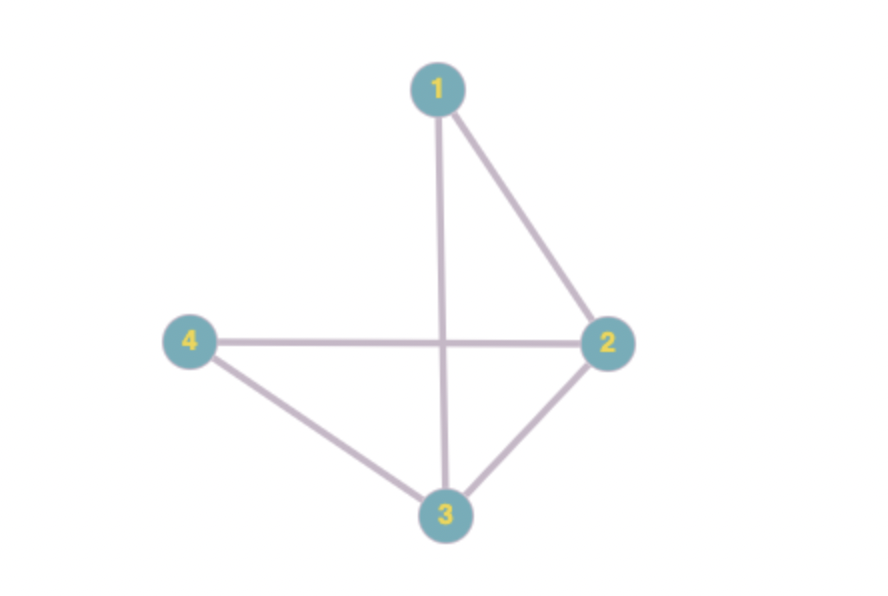
\includegraphics[scale=.35]{four_vertex.png}
    \caption{A 4-vertex graph $G$}
    \label{fig:four_vertex}
\end{figure}

\par Let $G$ be a graph with vertices $\{v_1,v_2,\dots,v_n\}$. To make a cut $\{S,\bar{S}\}$, we choose a subset of vertices $S$ such that both $S$ and its complement $\bar{S}$ are non-empty. There are $\stirlingtwo{n}{2}$ ways to do this. As $n$ increases, the increase in complexity of the problem accelerates greatly in what computer scientists often call a \textit{combinatorial explosion}. That is why the max-cut problem is $NP$-hard. \\

\par In the weighted version of max cut, a weight function $w(e_i)$ or $w(v_i,v_j)$ assigns a constant to each edge given by the vertex pair $v_i,v_j$ where $1\le i<j\le |V|$. Weights are more conveniently notated $w_{ij}$. They are often between 0 and 1, or non-negative at least. Vertex pairs with no edge are set to 0. For simplicity, we can think of an unweighted graph as a weighted graph with weights in $\{0,1\}$. The weight of a cut is the sum of the weights of the edges in it. In other terms, $w(S,\bar{S}) = \sum_{e\in (S,\bar{S})} w(e)$. \\

\par Now, for each vertex $v_i$, define the following:

$$y_i := \begin{cases}
    1 \quad &\text{if} \,\, v_i\in S \\
    -1 \quad &\text{otherwise.} \\
\end{cases}$$

\par It follows that the weight of the cut $(S, \bar{S})$ is given by $$w(S,\bar{S}) = \frac{1}{2}\sum_{i<j}  w_{ij}(1-y_iy_j).\footnote{If $v_i$ and $v_j$ are both in $S$ or $\bar{S}$, the corresponding term in this sum is 0. If, on the other hand, $v_i$ and $v_j$ are in different sets, the term contributes $w_{ij}$ to the sum. So the sum adds up the weights of only the edges that cross the cut.}$$ The edges whose weights maximize this function are the maximum cut of $G$. \\

\subsection{Example: Max Cut of a 4-Vertex Graph}

\par Consider the graph shown in Figure \ref{fig:four_vertex}. It has 4 vertices and thus only $\stirlingtwo{4}{2} = 7$ possible cuts, so we can easily check each one to see which contains the most edges. Table 1 gives the number of edges in each cut, which the reader can verify visually. The maximum cut, shown in Figure \ref{fig:four_vertex_cut}, separates vertices 1 and 4 from 2 and 3 and crosses a total of 4 edges. \\

\begin{figure}[!ht]
    \centering
    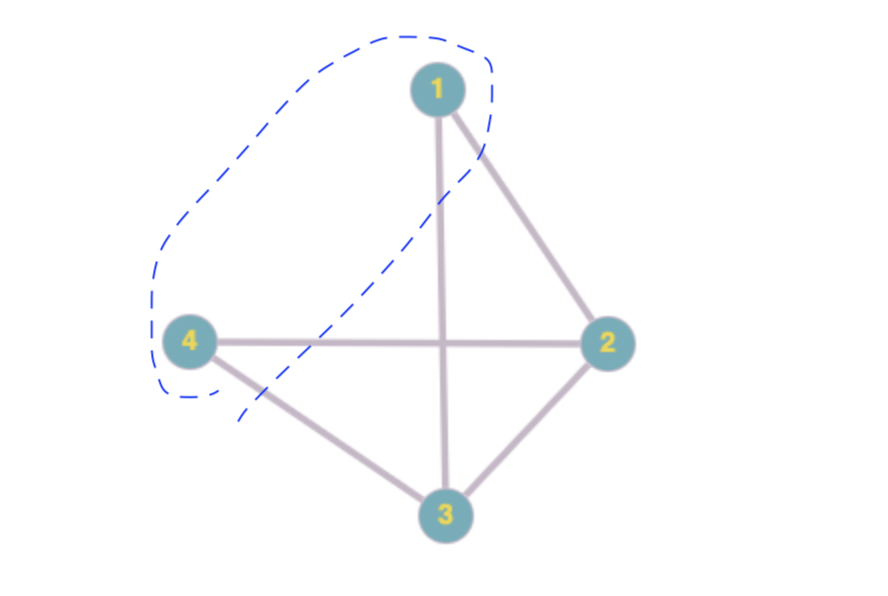
\includegraphics[scale=.35]{four_vertex_cut.png}
    \qquad
    \begin{tabular}[b]{|c|c|}
        \hline
        Cut & Size \\
        \hline
        $\{1,234\}$ & 2\\
        $\{2,134\}$ & 3\\
        $\{3,124\}$ & 3\\
        $\{4,123\}$ & 2\\
        $\{12,34\}$ & 3\\
        $\{13,24\}$ & 3\\
        $\{14,23\}$ & 4\\
        \hline
    \end{tabular}
    \captionlistentry[table]{A table beside a figure}
    \captionsetup{labelformat=andtable}
    \caption{The maximum cut of $G$}
    \label{fig:four_vertex_cut}
\end{figure}

\par What if we assign weights $w_{ij}$ to each edge, as shown in Figure \ref{fig:four_vertex_weighted_cut}? The maximum cut for this weighted graph is now $\{12,34\}$. Though it crosses fewer edges than $\{14,23\}$, its total weight is highest because its edges have relatively high individual weight compared to the rest. \\

\begin{figure}[!ht]
    \centering
    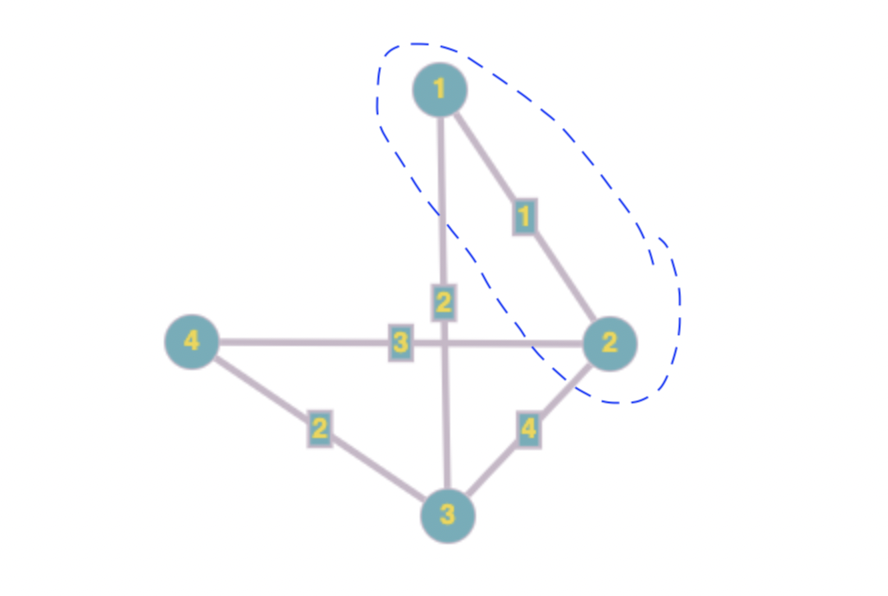
\includegraphics[scale=.35]{four_vertex_weighted_cut.png}
    \qquad
    \begin{tabular}[b]{|c|c|}
        \hline
        Cut & Size \\
        \hline
        $\{1,234\}$ & 3 \\
        $\{2,134\}$ & 8 \\
        $\{3,124\}$ & 8 \\
        $\{4,123\}$ & 5 \\
        $\{12,34\}$ & 9 \\
        $\{13,24\}$ & 7 \\
        $\{14,23\}$ & 8 \\
        \hline
    \end{tabular}
    \captionlistentry[table]{A table beside a figure}
    \captionsetup{labelformat=andtable}
    \caption{The maximum cut of weighted $G$}
    \label{fig:four_vertex_weighted_cut}
\end{figure}

\newpage

\subsection{Reformulating the Weight Function in Matrix Notation}

\par We can frame the problem in the language of linear algebra to more easily compute the weight of a given cut. Define the weight matrix $W := [w_{ij}]_{1 \le i \le n, 1 \le j \le n}$, and a cut as a binary vector $x$ of length $n$, where the $k$-th entry of $x$ is 1 if $v_k\in S$, 0 otherwise. Then the weight of the cut $x$ is given by $f(x) = x^T W(u-x)$, where $u$ is the length-$n$ vector of 1s. \\

\par We may now use a simple MATLAB program to compute the weight of a cut, shown in Figure \ref{fig:matlab_cut_weight_function}. \\

\begin{figure}[h]
    \centering
    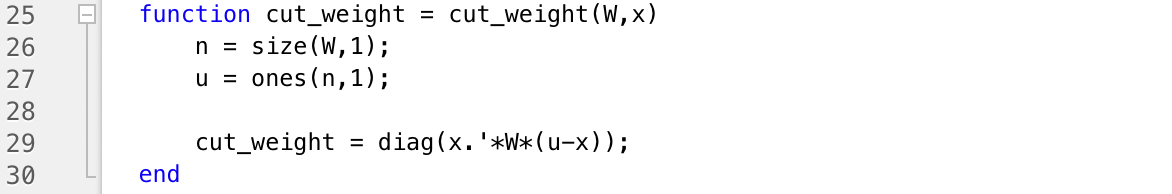
\includegraphics[scale=.5]{matlab_function.png}
    \caption{A MATLAB function that computes the weight of a cut $x$ given a weight matrix $W$}
    \label{fig:matlab_cut_weight_function}
\end{figure}

\par To save time, we can test multiple cuts at once by setting $x$ as a matrix with each column a cut. Then the $i$th entry of the output vector is the weight of the cut given by the $i$th column of $W$. Testing the function on our example above, Figure \ref{fig:matlab_four_vertex} shows that it returns the same answers we found earlier. \\

\begin{figure}[h]
    \centering 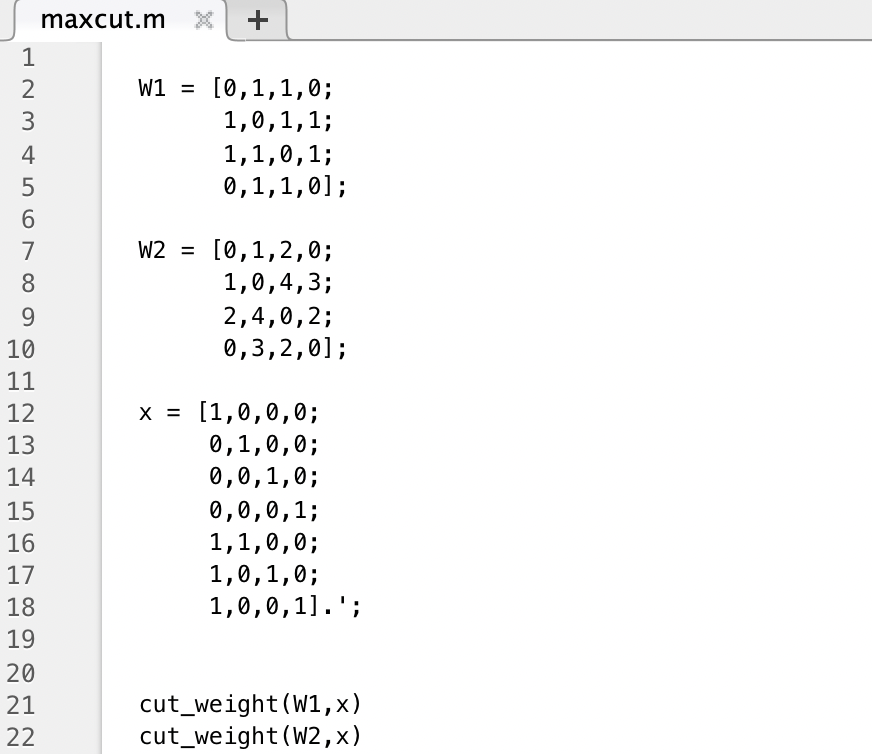
\includegraphics[scale=.5]{matlab_program.png}
    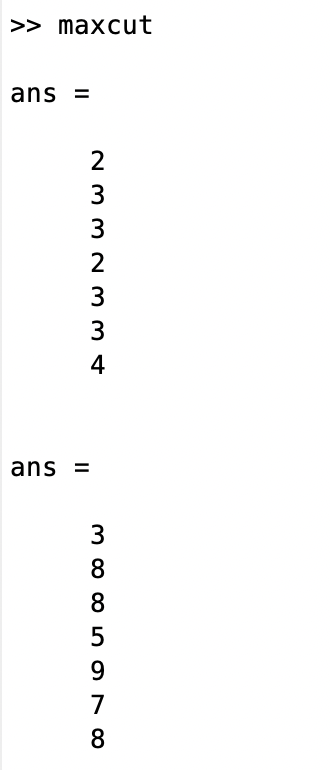
\includegraphics[scale=.5]{matlab_output.png}
    \caption{Computing the cuts from Example 2.1 with MATLAB}
    \label{fig:matlab_four_vertex}
\end{figure}